\chapter{Introduction}
	\lettrine[lines=4]{\color{activeColor}S}{uperfluids} are liquids and gases with remarkable properties. In particular, superfluid helium can flow through a capillary without friction due to its extremely small viscosity (at least 1500 times smaller than normal liquid helium\citep{Kapitza1938}), or creep up the wall of a container, seemingly defying the force of gravity\citep{Rollin1939} (``Rollin creeping''). Its thermal conductivity is about $3\times10^6$ times higher than that of liquid helium I or about 200 times higher than that of copper at room temperature\citep{Keesom1936}. It therefore earned the title of ``best heat conducting substance we know'' by Willem and his daughter Anna Keesom and dubbed ``\emph{supra-heat-conducting}''\citep{Keesom1936}. Later it was understood why\citep{Tisza1938-1,Tisza1938-2,Tisza1940-1,Tisza1940-2} and it turns out that heat does not diffuse through the medium as in normal liquids, but rather it travels through the medium in waves (second sound). This makes it an ideal coolant e.g. to stabilise the superconducting magnets in CERN's Large Hadron Collider\citep{Lebrun1994}. Helium is also the only known substance that stays liquid at zero temperature and low pressures and both its angular momentum and vorticity are quantised, making it the first observed macroscopic quantum substance. Helium-4 becomes superfluid below the $\lambda$-point, named so by William H. Keesom in 1936 who measured a singularity in the specific heat at $T_\lambda=2.2\unit{K}$\citep{Keesom1936}.
	
	\begin{figure}[t]
		\begin{center}
			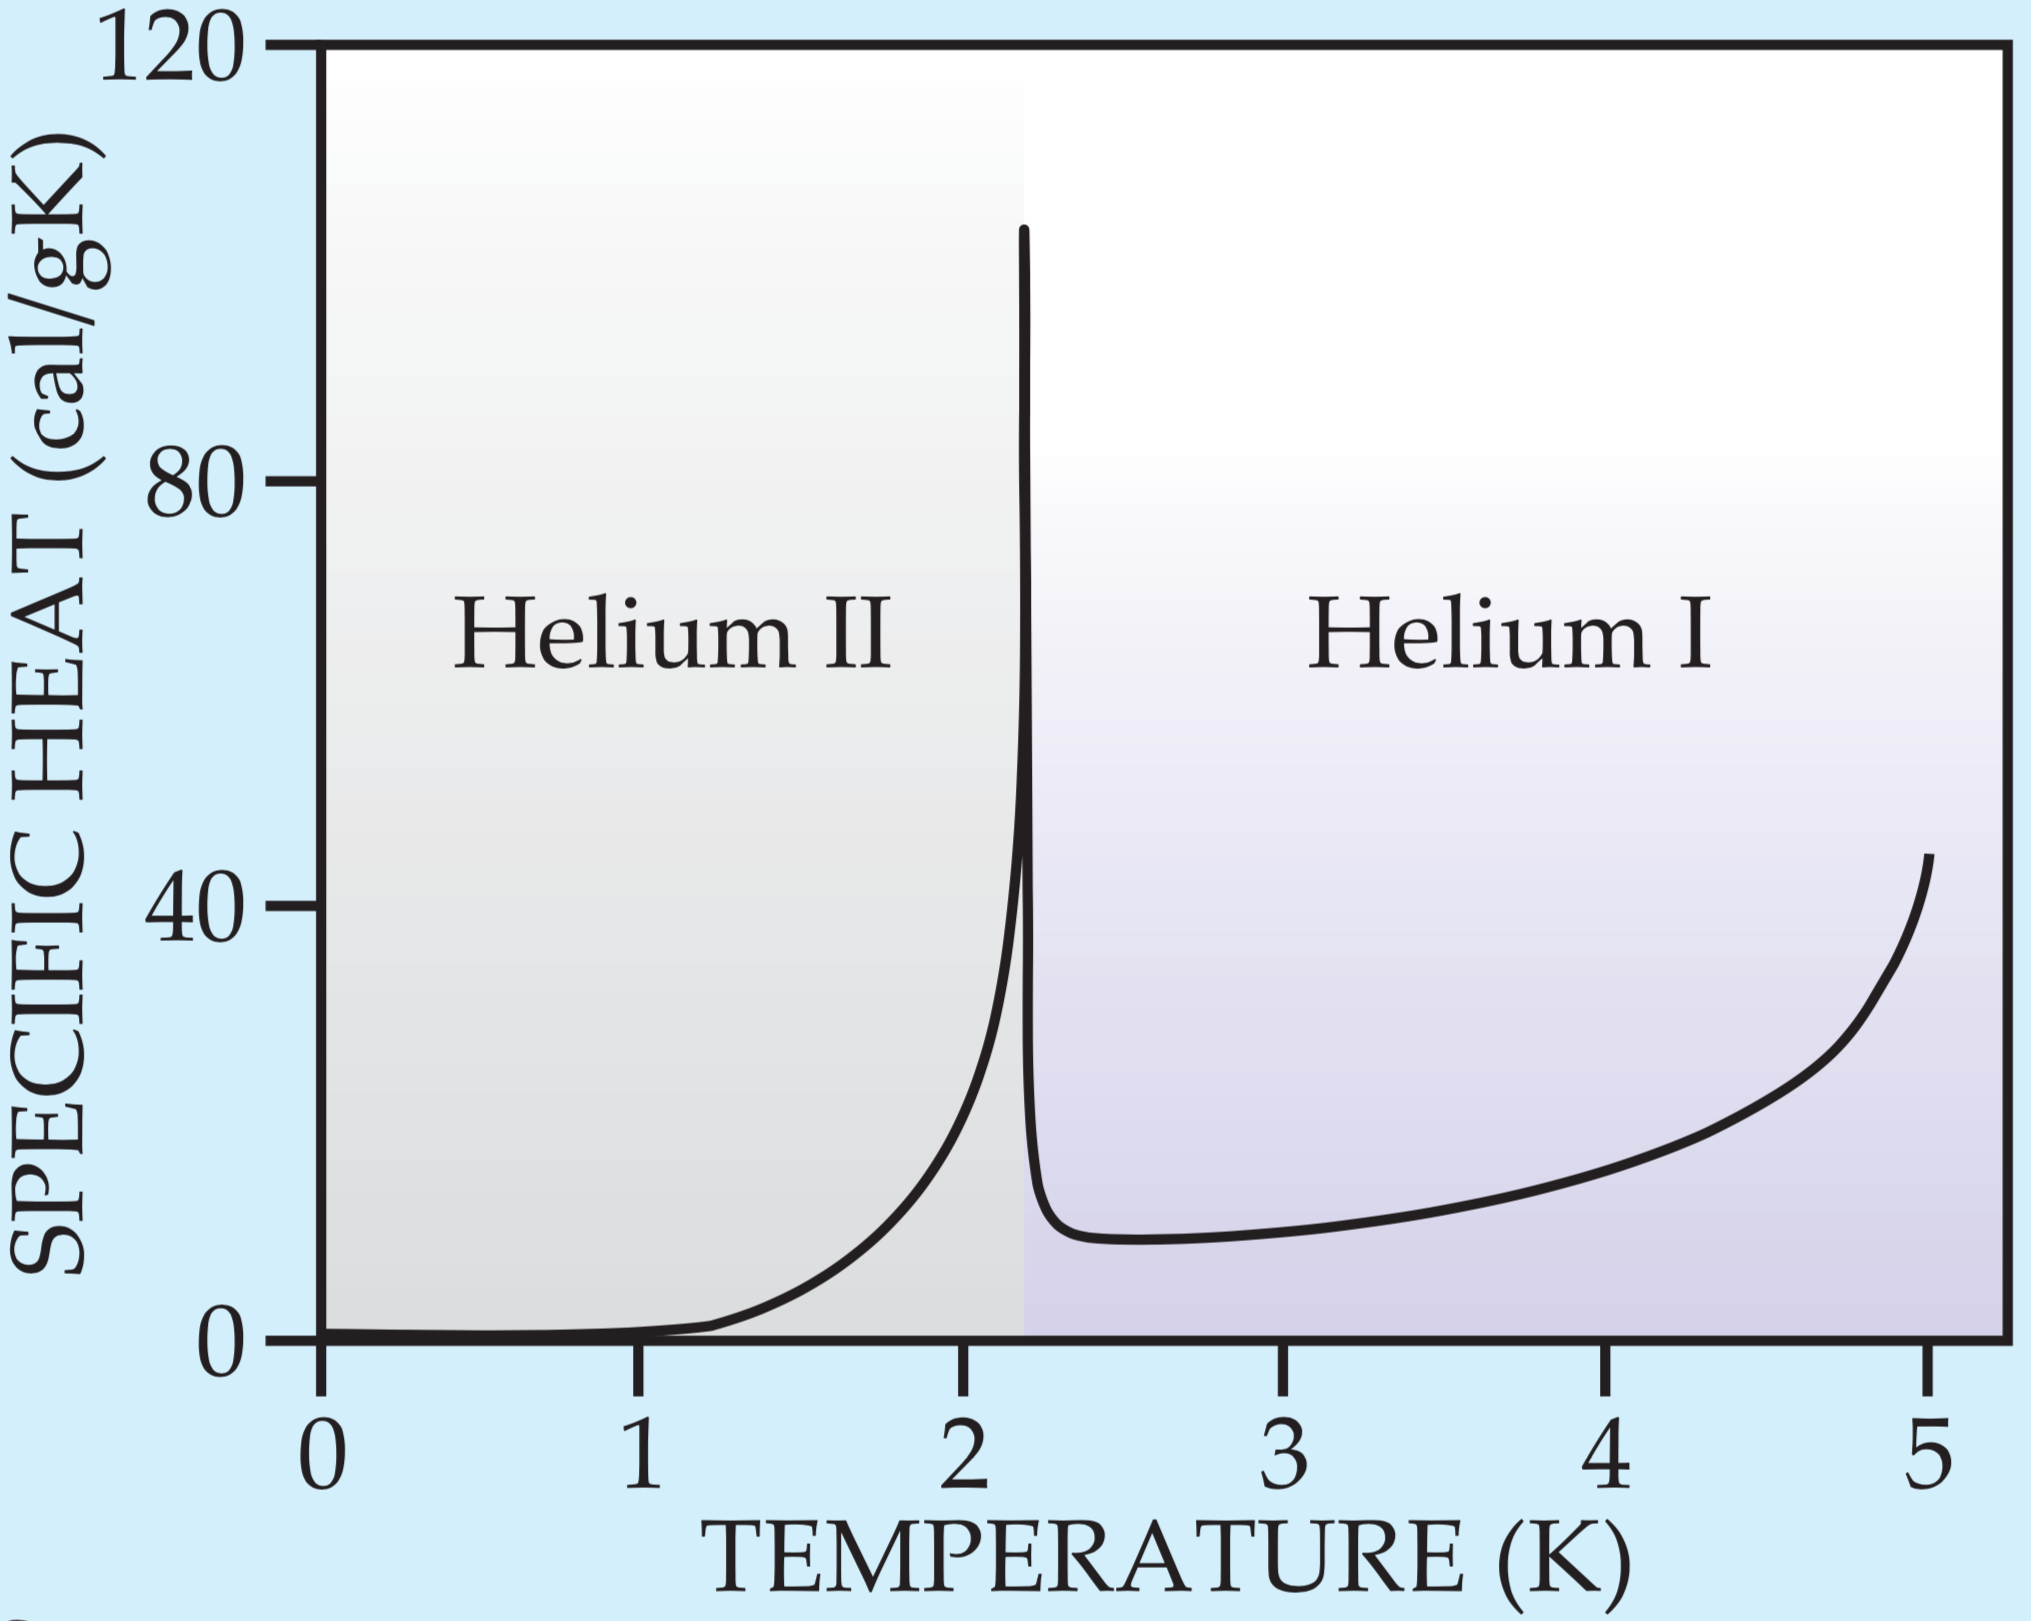
\includegraphics[width=0.75\textwidth]{specific-heat}
		\end{center}
		\caption{The specific heat of $^4$He as a function of the temperature. There is a clearly visible singularity around $2.2\unit{K}$ and the graph itself has the distinct $\lambda$-like shape that inspired\citep{Keesom1932} Willem and Anna Keesom to call the temperature at which the singularity occurs the ``$\lambda$-point''. (Illustration courtesy of R.J. Donnelly\citep{Donnelly2009})}
		\label{fig:specific-heat}
	\end{figure}	
	
	\section{A brief history of superfluidity}
		Helium was the last gas to be liquefied and was done so by Heike Kamerlingh Onnes in 1908\citep{Onnes1908,Onnes1909}. In 1932 John McLennan saw that liquid helium stopped boiling below $\sim$2.2~K\citep{McLennan1932} and later that year Willem Keesom and his daughter Anna observed, while measuring the temperature dependence of the specific heat, a singularity around the same temperature\citep{Keesom1932}. They called it the ``$\lambda$-temperature'',  $T_\lambda$, because of the shape of the temperature dependence of the specific heat resembling the Greek letter $\lambda$ (see \fig{fig:specific-heat}). A few years later in 1935 Burton measured a sharp decrease in the viscosity of liquid helium below $T_\lambda$\citep{Burton1935}. Around the same time Fritz London was already thinking about macroscopic wave functions and why helium does not freeze at $T=0\unit{K}$ under atmospheric pressure\citep{London1935}. London and Simon concluded that it was caused by the zero point motion of the helium atoms and their associated kinetic energy that is comparable to their Van der Waals energy, effectively preventing liquid helium to solidify\citep{Simon1934,London1936}. The year after, in 1936, Willem and Anna Keesom measured an abnormally high heat conductance below $T_\lambda$\citep{Keesom1936}. This was confirmed roughly one year later by J.F. Allen \emph{et al.}\citep{Allen1937} and it was understood that the high thermal conductance was the reason for the helium to stop boiling whenever the temperature drops below $T_\lambda$. It was in 1937, when Kapitza tried to determine the viscosity of the laminar flow, that he measured a viscosity that was about $10^4$ times smaller than that of hydrogen gas\citep{Kapitza1938}. It was then that Kaptiza, by analogy with superconductors, first coined the word ``superfluid''\citep{Kapitza1938} to describe the special state that helium enters below the $\lambda$-point where it can flow, seemingly without friction. Allen and Misener realised that superfluid helium is not just a liquid with a very low viscosity, but that its hydrodynamics was completely different from that of ordinary liquids\citep{Allen1938} and therefore required a completely new interpretation.

		A beginning to this new interpretation was made by London\citep{London1938} in 1938 when he made a connection between the behaviour of superfluid helium and that of an ideal ``Bose-Einstein'' (BE) gas. Both his calculated value for $T_c=3.09\unit{K}$ and the behaviour of the temperature dependence of the heat capacity for the ideal BE-gas were very similar to the measured ones for liquid helium below $T_\lambda$. He wrote to Nature that ``it was difficult not to imagine a connection with ``Bose-Einstein condensation'' (BEC). Tisza expanded upon London's ideas\citep{Tisza1938} and considered a Helium II system of total $N$ atoms to consist of two parts; a macroscopic ``condensed'' part $n_0$, the superfluid component, in the ground state, and the remaining part $n=N-n_0$, the normal component, where the helium atoms are distributed over the excited states. Assuming this was correct the fraction $n_0/N$ should decrease with increasing temperature according to the equation
		\begin{align}
			\frac{n_0}{N} = 1-\qty(\frac{T}{T_0})^s \quad \text{for} \quad T<T_0
		\end{align}
		where $s=3/2$ for an ideal gas and should be taken larger, e.g. $s=5$, for a real liquid with stronger interactions between the atoms.
				
		This was the birth of the ``two-fluid'' model. Within the framework of this model he derived two hydrodynamic equations for liquid helium below $T_\lambda$ and concluded that within superfluid liquid helium, heat propagates in waves instead of diffusing through the medium, and calculated the velocity of these waves. He also explained why the viscosity is disappearing at low temperatures contrary to classical liquids where the viscosity increases\citep{Tisza1938-1,Tisza1938-2,Tisza1940-1,Tisza1940-2}. In 1941 Lev Landau reformulated Tisza's theory on a more rigorous footing\citep{Landau1941,Landau1949}. He assumed, contrary to Tisza, that the normal component of the liquid was made-up of collective excitations instead of excited single atoms. He postulated that the liquid could exhibit two states of motion which he called ``potential motion'' that is irrotational ($\curl{\vec{v}}=0$), and ``vortex motion'' that is rotational ($\curl{\vec{v}} \neq 0$). The corresponding energies of these two motions are separated by an energy gap $\Delta$. In case of potential internal motion  the excitations are quanta of longitudinal (sound) waves, i.e., phonons. The excitations of the vortex-spectrum could be called ``rotons'' (see \fig{fig:phonon-roton}).

		\begin{figure}[t]
			\begin{center}
				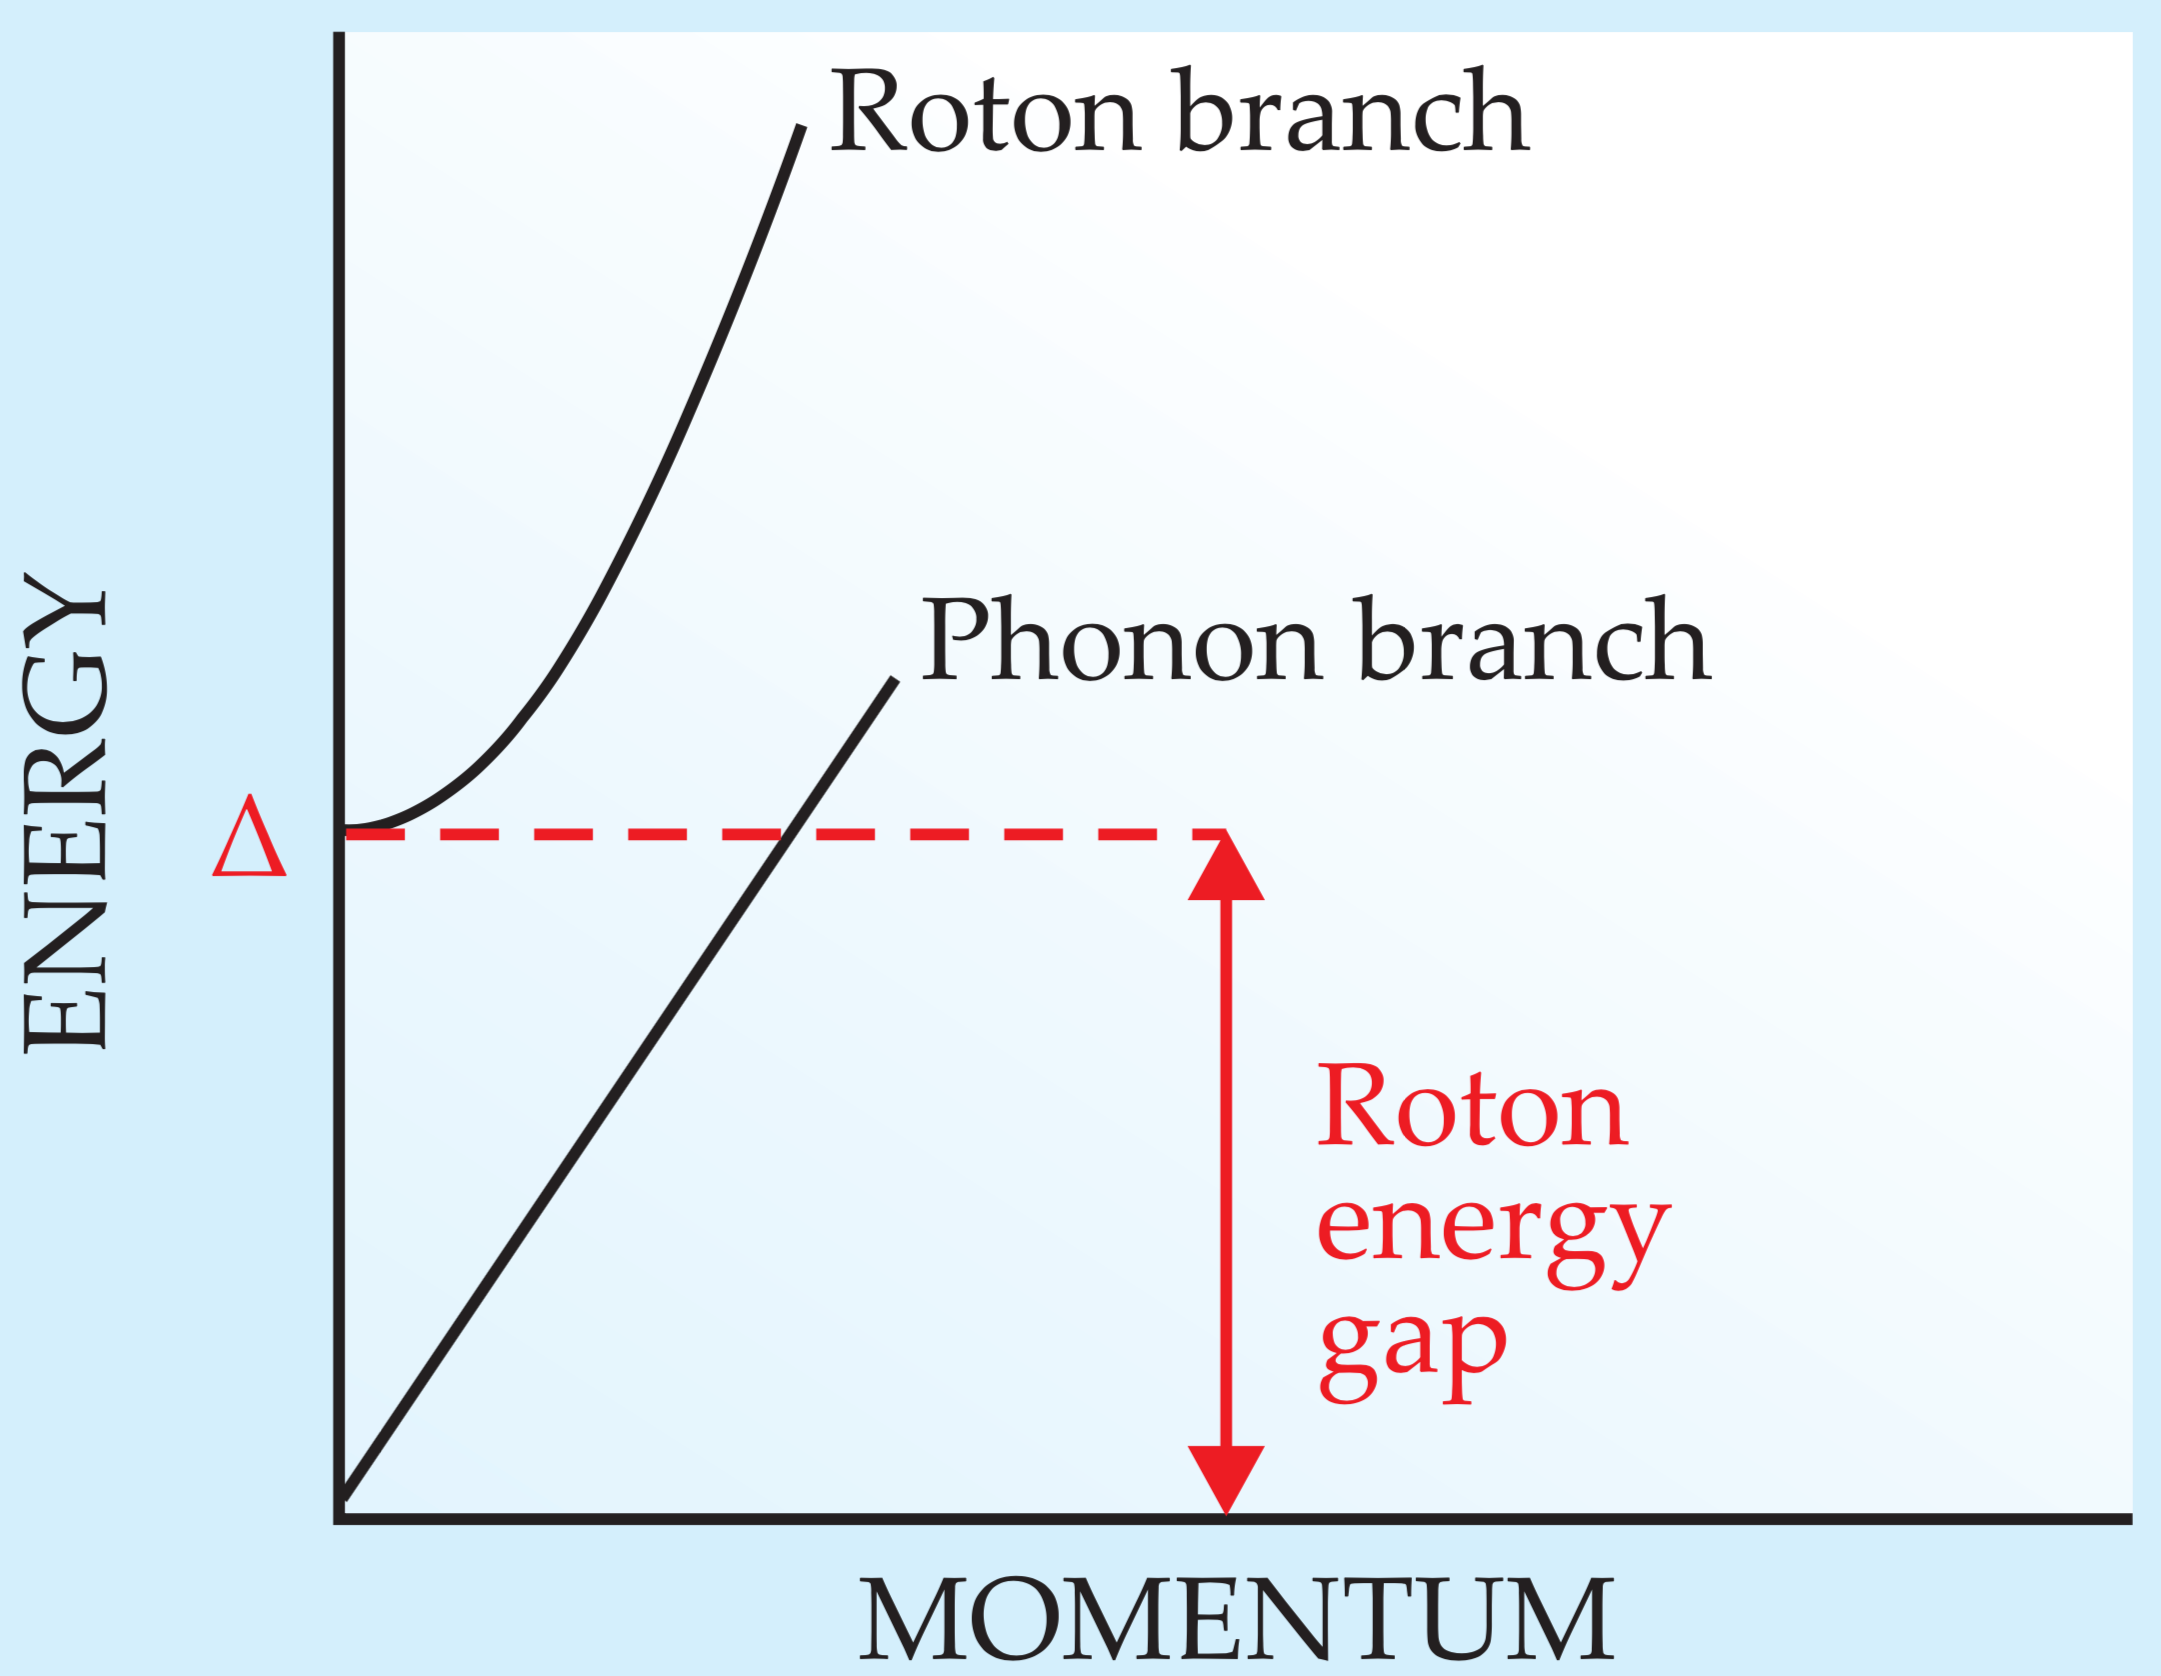
\includegraphics[width=0.490\textwidth]{phonon-roton-landau-first}\hspace{5pt}
				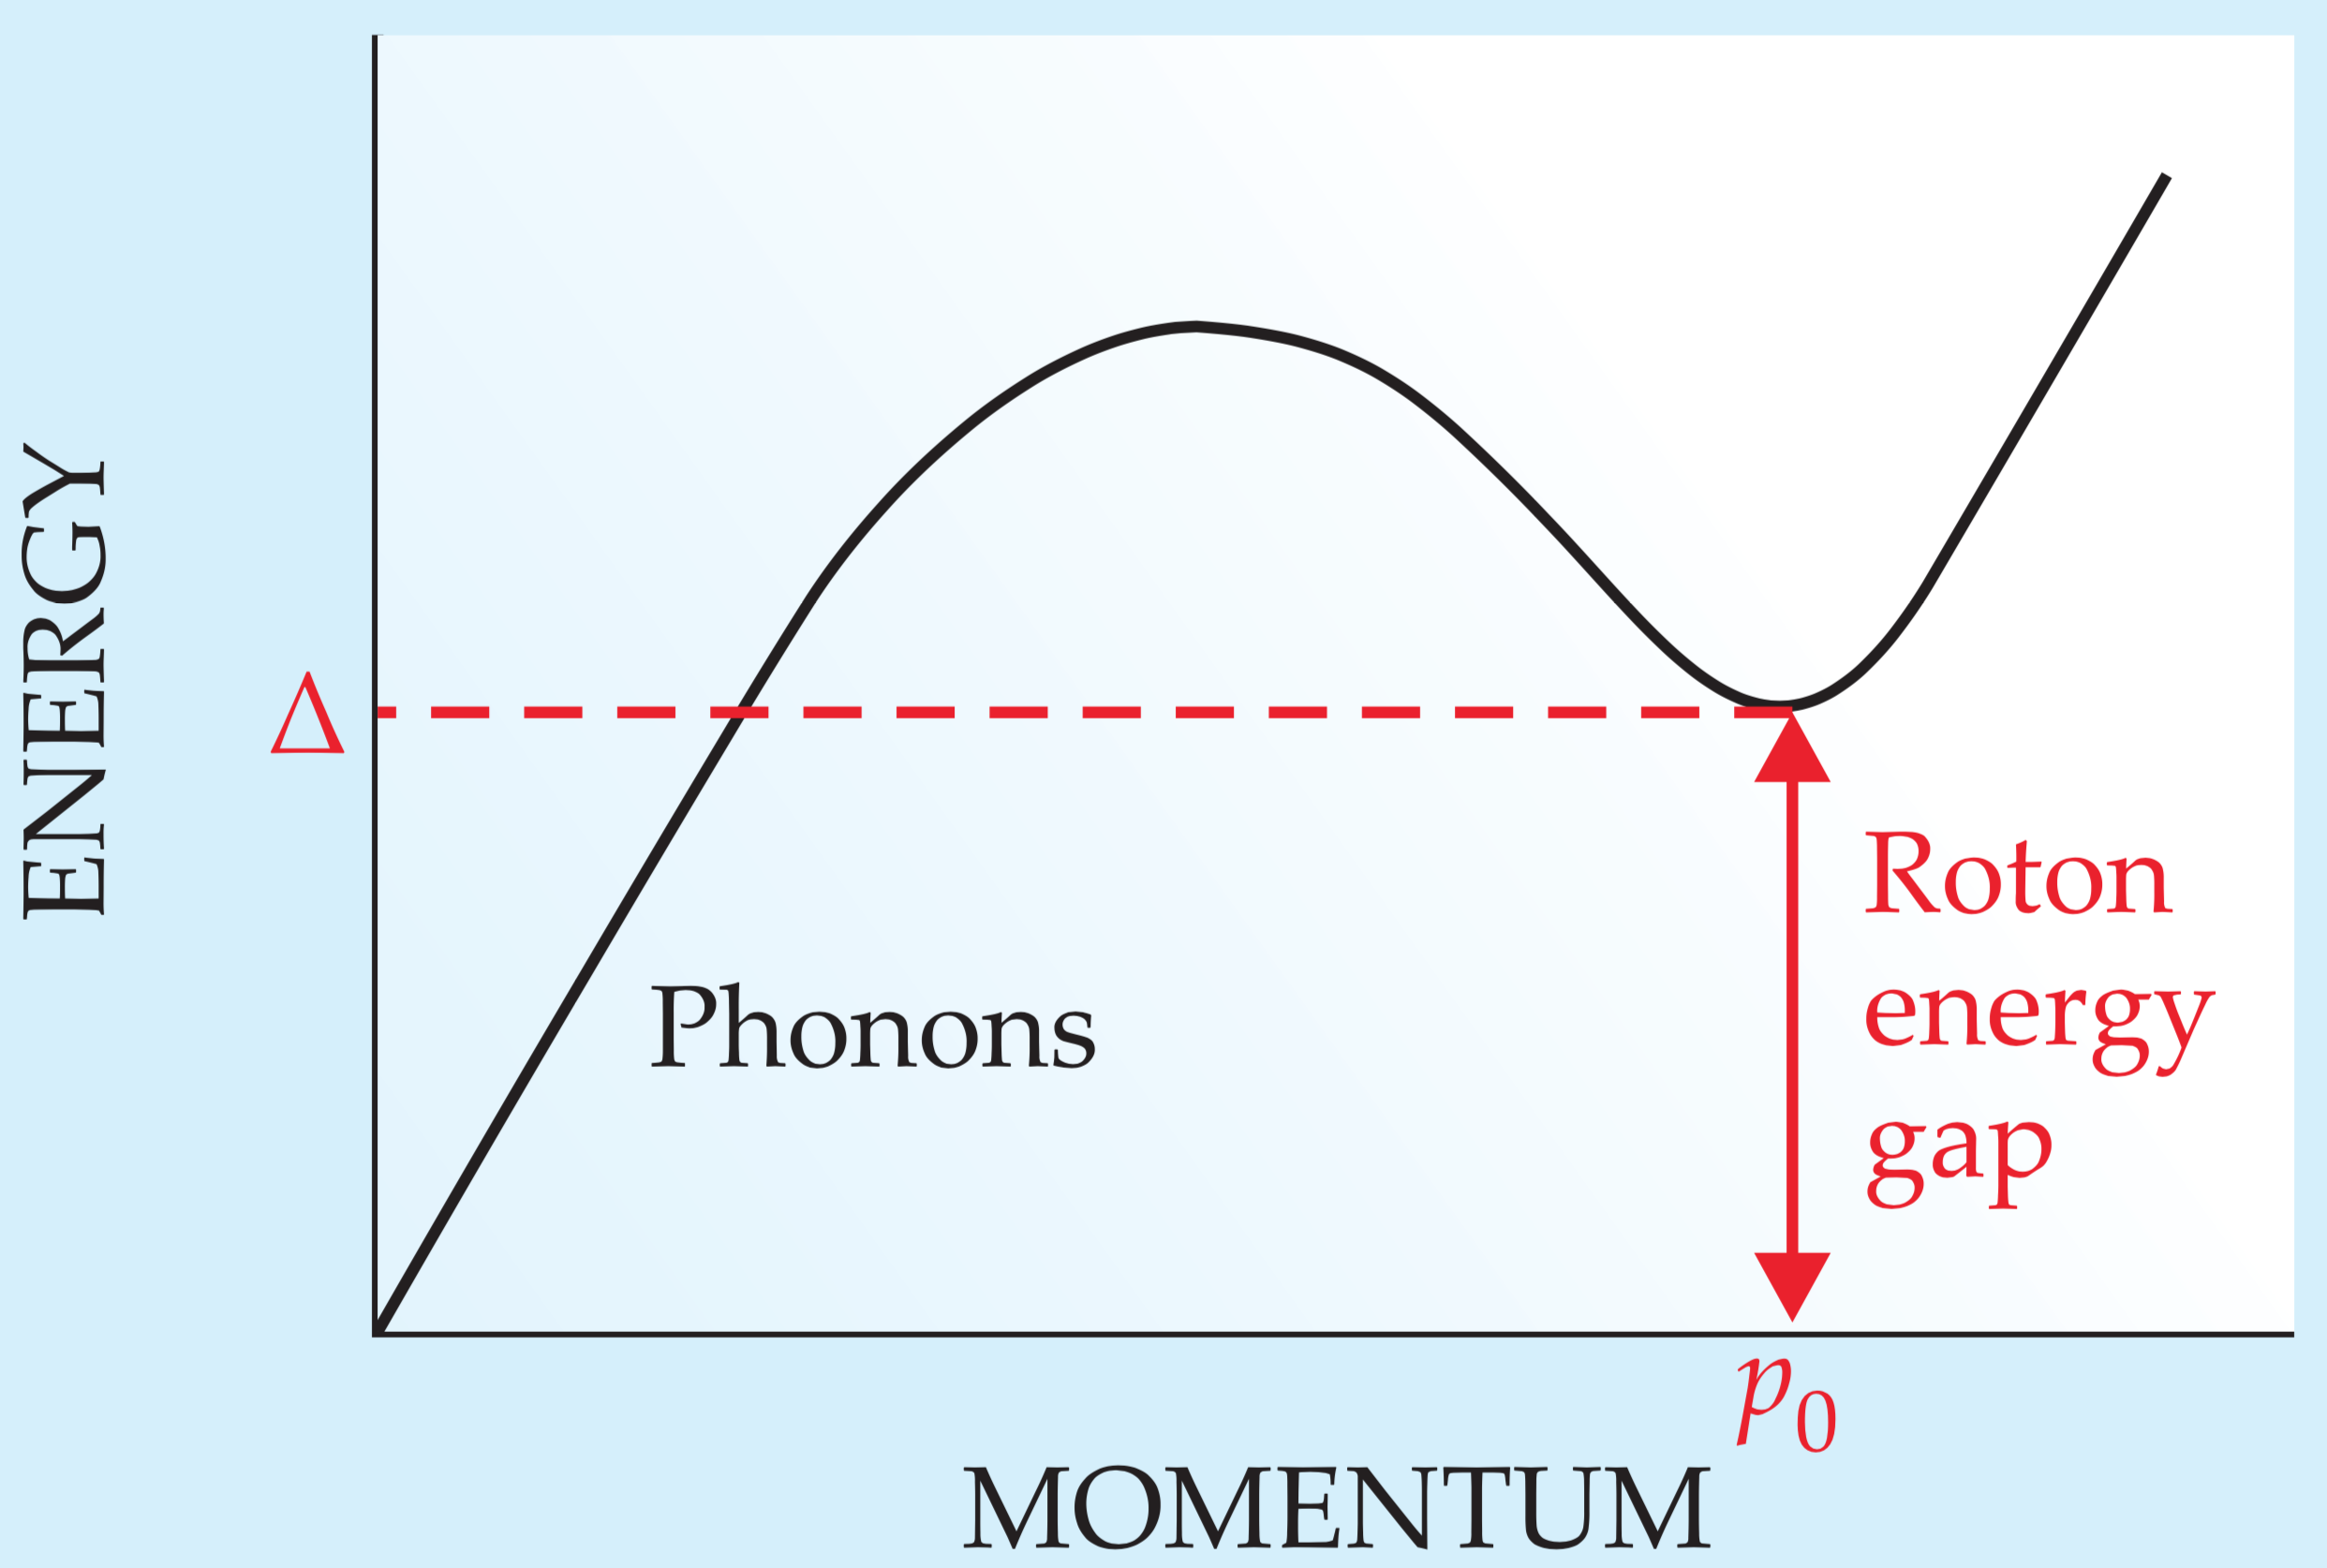
\includegraphics[width=0.490\textwidth]{phonon-roton-bogoliubov}
			\end{center}
			\caption{Left: Lev Landau's 1941 energy dispersion curve\citep{Landau1941} for the excitations in liquid helium below $T_\lambda$. It exhibits a phonon- and a roton branch. The slope of the linear phonon branch corresponds to the velocity of sound. Right: Lev Landau's 1947 modified dispersion curve. The roton-branch is no longer a separate excitation branch but rather an extension of the phonon-branch. (Illustration courtesy of R.J. Donnelly\citep{Donnelly2009})}
			\label{fig:phonon-roton}
		\end{figure}
		
		A theoretical demonstration, explicitly showing that phonons and rotons are collective excitations of the liquid, came in the form of a 1947 paper by Nikolay Bogolyubov\citep{Bogolyubov1947}. The intimate relationship between superfluidity and BEC was not universally accepted until 1995 when Cornell and Wienman in Colorado and Ketterle at MIT discovered BEC in rubidium quantum gases\citep{Cornell2002,Ketterle2002}.

	\section{Some key concepts}
		In this section I briefly introduce some key ideas that are used throughout the thesis and that are needed to fully appreciate the discussed material. Most of this introduction is guided by the work of Pitaevskii and Stringari\citep{Pita2016} on Bose-Einstein condensation. Also references to more complete and more in-depth treatments are provided for the interested reader.
		
		\subsection{Bose-Einstein condensation and long-range order}
			The essential concept of Bose-Einstein (BE) condensation is the fact that at low temperatures, multiple bosons, unlike fermions, occupy the same quantum state. In theory there is no upper bound on how many bosons can occupy such a single state. It is then said that, with ever decreasing temperature, a macroscopic part of the total number of bosons will ``condense'' into the quantum state with the lowest energy.		
			
			Another important concept in BEC is the idea of long-range order. Let us start by introducing the one-body density matrix of a system of $N$ bosons in a pure state $\Psi_k(\vec{r}_1,\vec{r}_2,\ldots,\vec{r}_N)$
			\begin{align}
				n^{(1)}_k(\vec{r},\vec{r'}) \vcentcolon= N\int\!	\Psi_k^*(\vec{r},\vec{r}_2,\ldots,\vec{r}_N)\Psi_k(\vec{r'},\vec{r}_2,\ldots,\vec{r}_N)\diff{r}_2\diff{r}_3\ldots\diff{r}_N	\label{eq:def-obd-matrix}
			\end{align}
			where the integral is taken over the $N-1$ coordinates $\vec{r}_2,\vec{r}_3,\ldots,\vec{r}_N$. For a statistical mixture of quantum states one needs to take the weighted average over all the different $\Psi_k$-states. At thermodynamic equilibrium the states are Boltzmann weighted by their eigenvalues $\qty{E_k}$
			\begin{align}
				n^{(1)}(\vec{r},\vec{r'}) = \frac{1}{Q}\sum_k n^{(1)}_k(\vec{r},\vec{r'}) \unit{e}^{-E_k/k_BT}
			\end{align}
			where $Q$ is the partition function. For more general cases the one-body density matrix is defined
			\begin{align}
				n^{(1)}(\vec{r},\vec{r'}) \vcentcolon=\expval{\hat\Psi^\dagger(\vec{r})\hat\Psi(\vec{r'})}
			\end{align}
			where $\hat\Psi^\dagger(\vec{r})$/$\hat\Psi(\vec{r})$ are field-operators creating/annihilating a boson at $\vec{r}$ and the averaging $\expval{\cdots}$ is taken over all states in the mixture. Once it is accepted that a macroscopic part of the total number of bosons can occupy a single quantum state it can be demonstrated that, while considering a uniform isotropic sytem of $N$ bosons, the one-body density matrix (\eq{eq:def-obd-matrix}) tends to a constant value when the distance between $\vec{r}$ and $\vec{r}'$ goes to infinity. In the thermodynamic limit where $N,V\rightarrow\infty$ such that $n=N/V$ is kept fixed, the one-body density only depends on the modulus of the relative variable $\vec{s}:=\vec{r}-\vec{r}'$ so that we can write it as the Fourier transform of the momentum distribution as
			\begin{align}
				n^{(1)}(s) = \frac{1}{V}\int \! n^{(1)}\qty(\vec{p})\exp(i\vec{p}\cdot\vec{s}/\hbar)\,\mathrm{d}\vec{p} \label{eq:one-body-den-mom}
			\end{align}
			For a BEC system, the momentum distribution at small momenta is not smooth but has a sharp peak around $p=0$ for the bosons that are in the ground state, while the remaining bosons are smoothly distributed over the excited states.
			\begin{align}
				n(\vec{p})=N_0\delta(\vec{p})+\tilde{n}(\vec{p})
			\end{align}
			where $\tilde{n}$ is a smoothly varying function of $\vec{p}$. When this expression is plugged into \eq{eq:one-body-den-mom} and taking the limit where $s$ goes to infinity it is obtained that
			\begin{align}
				\lim_{s\rightarrow\infty}n^{(1)}(s)=\frac{N_0}{V},
			\end{align}
			where $N_0/V \vcentcolon= n_0\leq 1$ is called the condensate fraction. It is called long-range order since it involves the off-diagonal elements of the one-body density matrix; the elements that are usually associated with the coherences.
			
			A set of eigenvalues \{$n_i$\} of the one-body density matrix can be defined through the following eigenvalue equation
			\begin{align}
				\int \! n^{(1)}(\vec{r},\vec{r'})\varphi_i(\vec{r'}) \,\mathrm{d}\vec{r'} = n_i\varphi_i(\vec{r})
			\end{align}
			and its solutions \{$\varphi_i$\} form a natural orthonormal basis set of single boson wave functions $\int\!\varphi_i^*\varphi_j\,\mathrm{d}\vec{r}=\delta_{ij}$, with normalisation condition $\sum_i n_i=N$. This permits writing the on-body density matrix in a useful diagonalised form. Recalling that BEC occurs when a single particle state $\varphi_i$ is occupied in a macroscopic way, say when $n_{i=0}=N_0$, a number of order $N$, we separate the condensate part from the rest
			\begin{align}
				n^{(1)}(\vec{r},\vec{r'}) = N_0\varphi_0^*(\vec{r})\varphi_0(\vec{r'})+\sum_{i\neq0}n_i\varphi_i^*(\vec{r})\varphi_i(\vec{r'}) \label{eq:obdm-diag}
			\end{align}

		\subsection{Bogolyubov's approximation}\label{sec:bogol-order}
			It is customary, given the importance of the condensate fraction $N_0$ in a BEC, to write the field operator of a $N$-body boson system as the sum of the condensate part and the rest, just as the one-body density matrix
			\begin{align}
				\hat{\Psi}(\vec{r})=\varphi_0(\vec{r})\hat{a}_0 + \sum_{i\neq 0} \varphi_i(\vec{r})\hat{a}_i \label{eq:field-operator}
			\end{align}
			where $\hat{a}_i$ and $\hat{a}_i^\dagger$ are the annihilation and creation operator of a particle in state $\varphi_i$ and obey the usual bosonic commutation relations
			\begin{align}
				\commutator{\hat{a}_i}{\hat{a}_j^\dagger}=\delta_{ij},\quad 	\commutator{\hat{a}_i}{\hat{a}_j}=0=\commutator{\hat{a}_i^\dagger}{\hat{a}_j^\dagger}
			\end{align}
			Using \eq{eq:field-operator} in \eq{eq:def-obd-matrix} and comparing it to \eq{eq:obdm-diag} one finds the expectation value of $\expectationvalue{\hat{a}_j^\dagger\,\hat{a}_i}=\delta_{ij}n_i$. Now, the Bogolyubov approximation essentially replaces the operators $\hat{a}_0$ and $\hat{a}_0^\dagger$ with the $c$-number\footnote{The term $c$-number is old nomenclature for a classical number, which can be real or complex, to distinguish them from quantum numbers, or $q$-numbers, that are represented by operators.} $\sqrt{N_0}$. This is equivalent to ignoring the non-commutative nature of the operators due to the macroscopic occupation of the state $\varphi_0$, when $N_0=\expectationvalue{\hat{a}_0^\dagger\,\hat{a}_0}\gg 1$. We then rewrite the field operator as the sum of a classical field for the condensed component and a quantum field for the non-condensed component
			\begin{align}
				\hat{\Psi}(\vec{r})=\Psi_0(\vec{r})+\delta\hat{\Psi}(\vec{r}),\label{eq:order-param-real}
			\end{align}
			where $\delta\hat{\Psi}(\vec{r})=\sum_{i\neq 0}\varphi_i(\vec{r})\hat{a}_i$ and $\Psi_0(\vec{r})=\sqrt{N_0}\varphi_0(\vec{r})$. At $T=0$ the whole system is condensed and one can ignore $\delta\hat{\Psi}$ altogether; the field operator becomes a normal function of space $\Psi_0$.
			
			The classical field $\Psi_0$ is called the \emph{effective}- or \emph{macroscopic} wave function of the condensate. It behaves like an order parameter in the sense that it represents the phase transition between the normal liquid phase and the superfluid phase. It varies continuously between the maximum value $\sqrt{N}$, which is proportional to the total number of bosons in the condensate at $T=0$, and vanishes at the superfluid/normal liquid phase transition temperature $T_\lambda$. It is a complex quantity characterised by a real-valued modulus and phase:
			\begin{align}
				\Psi_0(\vec{r}) = \absolutevalue{\sqrt{N_0}\varphi_0(\vec{r)}}\,\mathrm{e}^{iS(\vec{r})}\label{eq:order-param-complex}
			\end{align}
			The modulus determines the number-density of the condensate, while the phase $S$ plays an important role in the coherence and properties of the superfluid. As we will see in \scn{sec:rot-vort}, $S$ plays the role of a velocity potential.
			
			Using an order parameter as defined here is equivalent to using the many-body wave function
			\begin{align}
				\Phi(\vec{r}_1,\vec{r}_2,\ldots\vec{r}_N)=\prod_{i=1}^{N}\varphi_0(\vec{r}_i),
			\end{align}
			with a density operator $\hat{\rho}(\vec{r}) \vcentcolon= \sum_{i=1}^{N}\delta(\vec{r}-\vec{r}_i)$ (see \scn{sec:kohn-sham}). One way to see why this wave function plays the role of an order parameter is to look at its time dependence. For normal wave functions the time dependence is determined by the eigenvalues $E_i$ of the Hamiltonian of the system
			\begin{align}
				\Psi(\vec{r},t)=\psi(\vec{r})\,\mathrm{e}^{-iE_it/\hbar}
			\end{align}
			But in this case, the time dependence is determined by the chemical potential $\mu=E(N)-E(N-1)\approx \partial E/\partial N$
			\begin{align}
				\Psi_0(\vec{r},t)=\Psi_0(\vec{r})\,\mathrm{e}^{-i\mu t/\hbar} \label{eq:td-order-param}
			\end{align}
			Another aspect of $\Psi_0$ being an order parameter and not a true many-body wave function is that two solutions $\Psi_a$ and $\Psi_b$ of the non-linear droplet Hamiltonian corresponding to two different values of the chemical potential $\mu_a$ and $\mu_b$ are not necessarily orthogonal, i.e. $0 \leq N^{-1}\int\!\Psi_a^*\Psi_b\unit{d}\vec{r} < 1$.% However, in dilute gases it is possible to construct a many-body wave function from the order parameter that regains its orthonormality in the thermodynamic limit
%			\begin{align}
%				\Phi_0(\vec{r}_1,\vec{r}_2,\ldots,\vec{r}_N) = \qty(\frac{1}{\sqrt{N}}\Psi_0(\vec{r}_1))\qty(\frac{1}{\sqrt{N}}\Psi_0(\vec{r}_2))\cdots\qty(\frac{1}{\sqrt{N}}\Psi_0(\vec{r}_N))
%			\end{align}
			
		\subsection{Landau's criterion for superfluidity}
			\begin{figure}[t]
				\begin{center}
					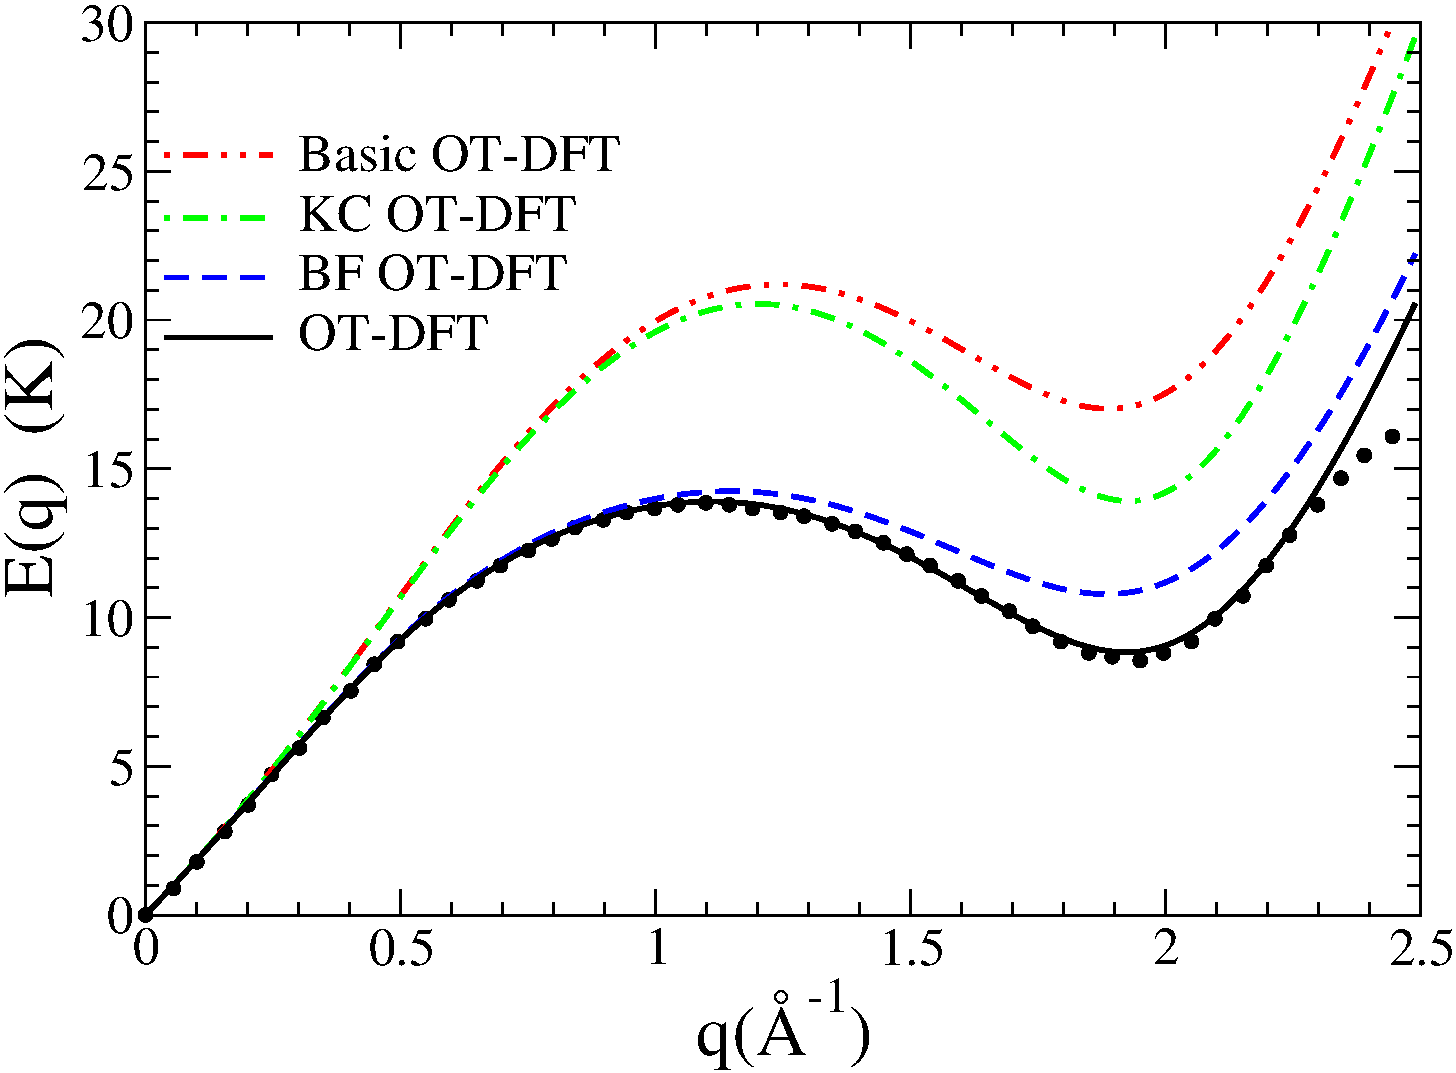
\includegraphics[width=0.75\textwidth]{dispersion-relation}
					\caption{Dispersion relation for elementary excitations in liquid $^4$He calculated as in  \cite{Mat10a}. `Basic' indicates the Orsay-Trento (OT) functional\citep{Dalfovo1995} without the non-local kinetic energy correction (KC) nor the back-flow (BF) terms; KC OT-DFT adds to the basic OT-DFT the KC term; BF OT-DFT adds to the basic OT-DFT the BF term. The dots are the experimental data from \cite{Don81}. The Landau velocity $v_L = E(q)/(\hbar\,q)|_{min}$ obtained for each functional is 60.3 m/s (OT-DFT); 75.1 m/s (BF OT-DFT); 94.4 m/s (KC OT-DFT); 118 m/s (basic OT-DFT); and 57.5 m/s (experiment). See also \scn{sec:otdft}.}
					\label{fig:dispersion-relation}
				\end{center}
			\end{figure}
		
			For a gas or liquid to be able to become superfluid Landau postulated that the energy dispersion relation needs to fulfil certain requirements. Specifically for a fluid to flow  without dissipation, i.e. a super-flow, the velocity field needs to fulfil the following inequality:
			\begin{align}
				v<v_c = \min_{\vec{p}}\frac{\epsilon(\vec{p})}{p}
			\end{align}
			
			For an ideal Bose gas $\epsilon(\vec{p})= \frac{p^2}{2m}$. In this case 
			\begin{align}
				v_c &= \min_{\vec{p}}\frac{\epsilon(\vec{p})}{p} \\
					&= \min_{\vec{p}}\frac{p}{2m} \\
					&= 0
			\end{align}
			Apparently an ideal Bose-gas cannot become superfluid.
			
			But if we allow for some weak interactions between the bosons the energy dispersion relation is given by
			\begin{align}
				\epsilon(\vec{p})=\sqrt{\frac{gn}{m}p^2+\qty(\frac{p^2}{2m})^2},
			\end{align}
			Bogolyubov's dispersion law for elementary excitations (1947). And thus
			\begin{align}
				v_c &=\min_{\vec{p}}\sqrt{\frac{gn}{m}+\frac{p^2}{4m^2}} \\
					&= \sqrt{\frac{gn}{m}} \\
					&= c,
			\end{align}
			the speed of sound. Here $g=\frac{4\pi\hbar^2a}{m}$, and $a$ the $s$-wave scattering length. The weakly interacting Bose gases can become superfluid.			

			Liquid helium below the $\lambda$-point has a similar energy dispersion relation (see \fig{fig:dispersion-relation}) hence reinforcing the notion that superfluidity and Bose--Einstein condensation are two intimately related concepts. The experimental value of the speed of sound in bulk superfluid liquid helium is $\sim$57.5~m/s.
			
		\subsection{Rotation and vorticity in superfluids}\label{sec:rot-vort}
			\begin{figure}[t]
				\begin{center}
					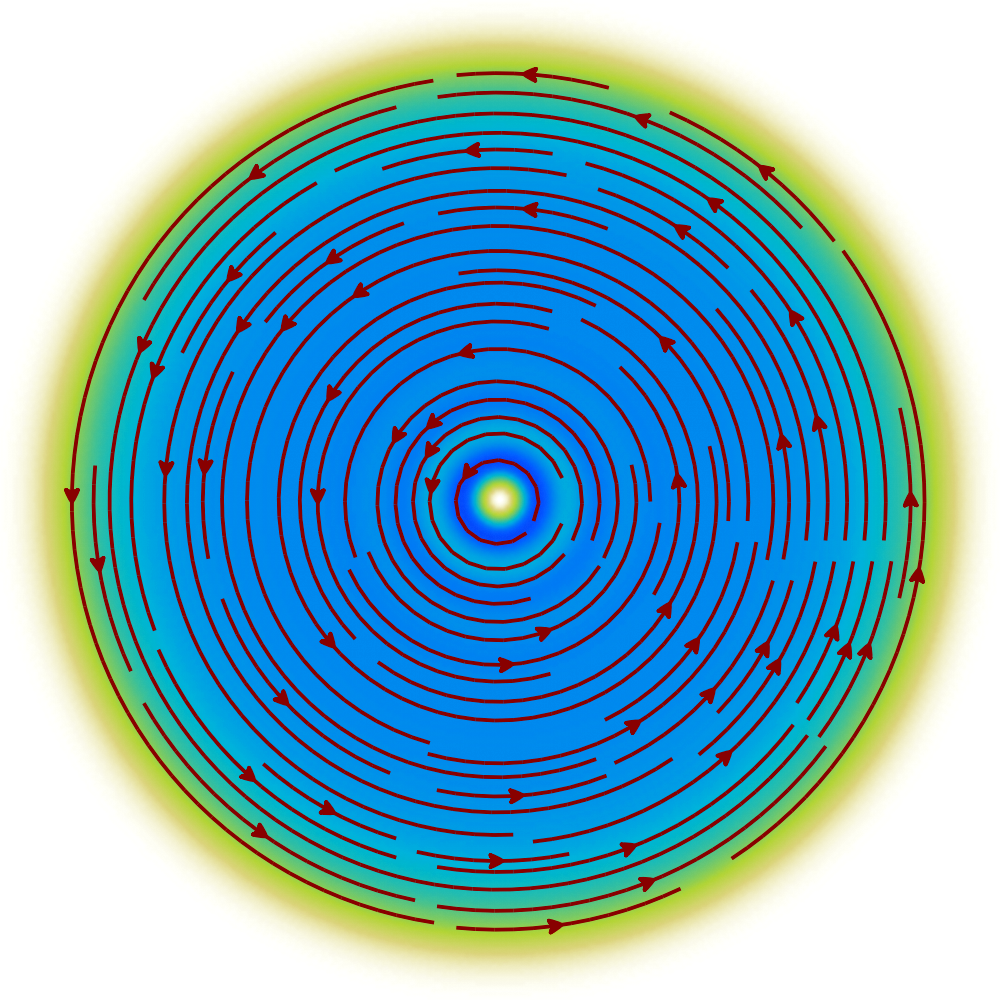
\includegraphics[width=0.75\textwidth]{vortex-xy-inverted-color}
					\caption{Cross section of a $^4$He droplet through a symmetry plane. The droplet is made of 1000 atoms. Superimposed are the streamlines of the velocity field $\vec{v}_s$ for $s=1$. They are concentric circles, centred around the vortex core along the $z$-axis. The colour scale represents the the number density $\rho(r)$ where bluer means a higher value. The radius of the droplet is about 22\,\AA.}
					\label{fig:vortex-xy}
				\end{center}
			\end{figure}
		
			We introduce here the concept of quantised vortices in the DFT approach. It will be shown later in \scn{sec:tddft} that within the DFT framework, the order parameter $\Psi$ is a solution of the time-dependent Euler-Lagrange (EL) \eq{eq:el-equation}. Taking this for grated for now, lets start with \eq{eq:el-equation} and the order parameter from \eq{eq:order-param-complex}, dropping the ground-state subscript and allowing $\varphi$ and $S$ to vary in time
			\begin{align}
				i\hbar\frac{\partial}{\partial t} \Psi({\mathbf r},t) = \left[-\frac{\hbar^2}{2m}\laplacian + \frac{\delta{\cal E}_{c}}{\delta\rho}\right]\Psi(\textbf{r},t)
			\end{align}
			one left-multiplies it with the complex conjugate of the order parameter $\Psi^*$ and then subtract the complex conjugate of the whole expression on both sides. After some algebra and defining $\rho(\vec{r},t)\vcentcolon=N\abs{\varphi(\vec{r},t)}^2$, one arrives at the continuity equation
			\begin{align}
				\frac{\partial\rho}{\partial t} + \div{\vec{j}}=0, \label{eq:continuity-eq}
			\end{align}
			with
			\begin{align}
				\vec{j}(\vec{r},t) \vcentcolon=& -\frac{i\hbar}{2m}\qty\big[\Psi^*(\vec{r},t)\grad{\Psi}(\vec{r},t) - \Psi(\vec{r},t)\grad{\Psi^*}(\vec{r},t)] \\
					=&\,\rho(\vec{r},t)\frac{\hbar}{m}\grad{S(\vec{r},t)}
			\end{align}
			From \eq{eq:continuity-eq} it follows that the atomic number density is a conserved quantity.
			
			We can identify the collective velocity $\vec{v}_s$ of the superfluid through the relation
			\begin{align}
				\vec{v}_s(\vec{r},t) = \vec{j}/\rho=\frac{\hbar}{m}\grad{S(\vec{r},t)} \label{eq:velocity-field}
			\end{align}
			and we see that the rotation of the velocity field of the superfluid $\curl{\vec{v}_s}=0$, i.e. the fluid is said to be \emph{irrotational}; a typical property of superfluids. Conversely, taking the curl $\curl{\vec{j}}=\frac{\hbar}{m}\grad{\rho}\times\grad{S}$ we see that this is merely a restatement of the fact that one needs a gas or liquid with a non-uniform density and a non-zero phase for it to be able to support vortices. The fact that a vortex in the gas or liquid exists directly implies $\grad{\rho}\neq 0$.
			
			Let us consider the illustrative example of a line vortex through the origin along the $z$-axis. As will be demonstrated in \scn{sec:vortical-states}, this is a stationary state of the droplet Hamiltonian and therefore its time dependence is just a multiplicative factor. In cylindrical coordinates $(r,\varphi,z)$ such a vortex solution has the form
			\begin{align}
				\Psi_s(\vec{r}) = \sqrt{\rho(r,z)}\unit{e}^{is\varphi}, \label{eq:line-vortex}
			\end{align}
			with $s$, the angular momentum, an integer. This is an eigenfunction of the angular momentum operator $\hat{L}_z$ with eigenvalue
			\begin{align}
				\hat{L}_z \Psi_s(\vec{r}) &= \frac{\hbar}{i}\frac{\partial}{\partial\varphi}\Psi_s(\vec{r}) = \hbar s\Psi_s(\vec{r})
			\end{align}
			and with expectation value
			\begin{align}
				\expval{\hat{L}_z} &= \expval{\hat{L}_z}{\Psi_s} \\
					&= \hbar s \braket{\sqrt{N_0}\varphi_0} \\
					&= N_0\hbar s
			\end{align}
			The angular momentum is quantised in units of $\hbar$ and proportional to the number of bosons in the BEC fraction/superfluid. We can calculate the velocity field
			\begin{align}
				\vec{v}_s = \frac{\hbar}{m}\grad{S} = \frac{\hbar}{m}\frac{s}{r}\,\vu*{\varphi}
			\end{align}
			The streamlines of $\vec{v}_s$ are concentric circles, centred around the z-axis, lying in the $xy$-plane (see \fig{fig:vortex-xy}). Contrary to rigid rotation fields which increase proportional to the distance from the $z$-axis $r$, the superfluid rotation field decreases proportional to the inverse of the distance from the $z$-axis $1/r$ and is singular in the origin. Calculating the circulation of the velocity field $\vec{v}_s$ along a closed contour including the $z$-axis gives
			\begin{align}
				\oint_{\partial\Sigma}\!\vec{v}_s\cdot\unit{d}\vec{l} &=
				\int_{0}^{2\pi}\!\frac{\hbar}{m}\frac{s}{r}\,\vu*{\varphi}\cdot r\unit{d}\varphi\,\vu*{\varphi} \\
					&= s\frac{h}{m}
			\end{align}
			where $h=2\pi\hbar$ is Planck's constant. There are two things to note here. Firstly, the circulation around a closed loop that encompasses the $z$-axis is quantised in units of $h/m$ for $s\in\mathbb{N}_{>0}$. Secondly, the value of the circulation of the velocity field does not depend on the chosen contour as long as it includes the location of the vortex. This means that all the vorticity is contained at the location where the velocity field is singular (the ``core'' of the vortex), at $r=0$ along the $z$-axis.
			
			Because of the pole in the velocity field, Stokes' theorem will lead to the following contradiction
			\begin{align}
				s\frac{h}{m}=\oint_{\partial\Sigma}\!\!\!\vec{v}_s\cdot\unit{d}\vec{l} = \iint_{\Sigma}\!\curl{\vec{v}_s}\cdot\unit{d}\vec{\Sigma} = 0
			\end{align}
			and can therefore not be applied. To emphasise that all the vorticity is concentrated around the vortex core one can write formally
			\begin{align}
				\curl{\vec{v}_s} = s\frac{h}{m}\delta^{(2)}(\vec{r}_\perp)\,\vu{z},
			\end{align}
			where $\delta^{(2)}$ is 2-dimensional Dirac-delta function and $\vec{r}_\perp$ a vector in a plane perpendicular to the vortex line.

	\section{Helium droplets}\label{sec:helium-droplets}
		Until the 1980's, most experimental and theoretical work was done on bulk systems, i.e. systems of the order of $N_A$ number of atoms. It was only in the last couple of decades that advancements in technology enabled experimentalists to create nanoscale sized superfluid helium droplets. From the early 1990's onwards, superfluid helium nano-droplets became an active field of study, both experimentally and theoretically. 
		
		Helium nanodroplets are considered ideal model systems to explore quantum hydrodynamics in self-contained, isolated superfluids. The main focus has been on the evolution of their properties with the number of atoms in the cluster, until the condensed matter limit is reached. Helium clusters are especially interesting in that quantum effects play a key role in determining their properties. In particular, given that a helium cluster is an ensemble of bosons at about 0.4 K\citep{Brink1990,Hartmann1995}, manifestations of collective behaviour (such as superfluidity) are expected. On the other hand, it is not yet clear how the finite size of a cluster affects this non-classical (or degenerate) collective behaviour.

		Recently, Toennies et al.\citep{Hartmann1996} have measured the electronic spectrum of glyoxal molecules embedded in He clusters and found it consistent with a theoretical simulation computed using the phonon dispersion curve of superfluid bulk He II. The authors themselves, however, point out that at the average cluster size of 5500 He atoms reported in\rf{Hartmann1996}, the clusters are so big that finite size effects in the interior region are negligible (see also\rfs{RamaKrishna1990-1,Chin1992}). It is therefore not surprising that they find results consistent with the bulk case, especially for a molecule readily solvated inside the cluster, for which surface effects play a minor role. Therefore the influence of the He clusters size on superfluidity has not been detected so far.
		
		The helium-helium interaction is already weak in bulk liquid helium and in finite self-bound systems such as droplets it is even weaker, e.g. the binding energy per atom is $<$7.17~K. Because of this helium droplets cool down very rapidly due to fast evaporation and therefore reaching their limiting temperature of about $0.38\unit{K}$ in microseconds. Pure helium droplets are neutral systems and their properties like their size, binding energy and excitation spectra, are not easy to determine experimentally and are usually obtained by indirect methods. This did not stop the theoreticians describe doped $^4$He$_N$ droplets using a wide variety of approaches depending on the size and character of the droplets ranging from Quantum Monte Carlo, Hypernetted-Chain/Euler-Lagrange\citep{Krotscheck2001}, Variational Monte Carlo\citep{Gartner2018} and many others.
		
		A key property of helium droplets, in contrast to bulk helium, is their ability to pickup any kind of dopants with which they collide. Depending on the strength of the dopant-$^4$He interaction and the surface tension of the droplet, a dimensionless parameter $\lambda$ can be defined\citep{Anc95} with a critical value $\lambda_0\sim1.9$. Below $\lambda_0$ impurities are bound to the surface of the droplet (e.g. the alkalis), and above they get solvated into the droplet's interior. Droplets can therefore be doped with almost any kind of atomic- or molecular species. 
		
		From the perspective of the droplet it this means that it is possible to use the dopants as gentle probes to determine the superfluid properties of helium droplets that would be inaccessible with other methods. For two examples of this see\rfs{Gre98,Sin89,RamaKrishna1990-2}, where a dopant is used to probe the superfluid character of small $^4$He droplets and\rfs{Hartmann1999,Harms1999} to see their limiting temperatures.
		
		Moreover, from the perspective of the impurities it enables a broad spectrum of possible experimental studies. Due to the fact that helium droplets are ultra cold superfluid liquids, and therefore provide high mobility of any picked-up dopants, one can conduct high resolution spectroscopy studies. Having a fine control over the number of picked-up dopants[29] one can use droplets as a matrix for creating self-organising structures of polar molecules, or very cold metal clusters and study their Coulomb explosion.
				
		\begin{figure}[t]
			\begin{center}
				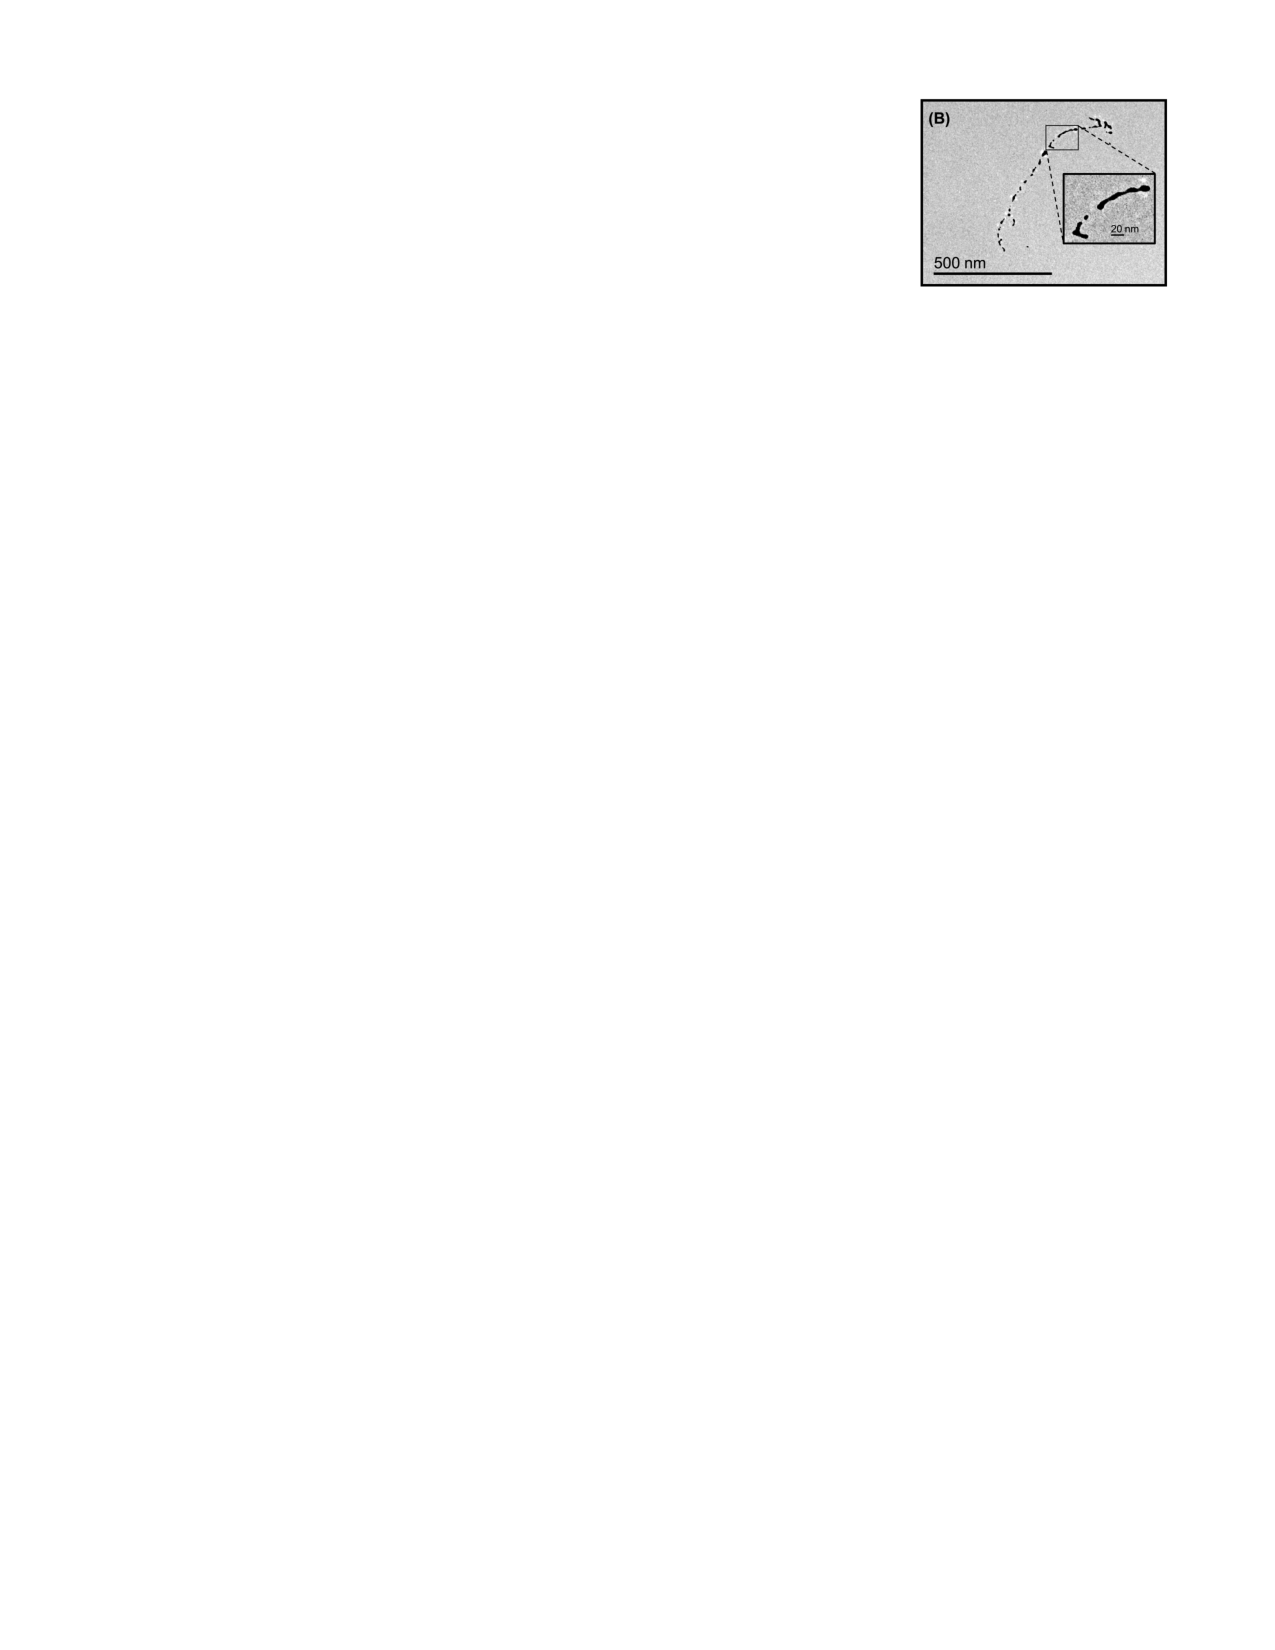
\includegraphics[width=0.75\textwidth]{silver-filament}
				\caption{Electron-microscope image of and elongated track-shaped Ag-cluster after it is surface-deposited.}
				\label{fig:silver-filament}
			\end{center}
		\end{figure}	
				
		One of the most intriguing properties of superfluid helium droplets is the fact that they can host quantised vortices. Because of their ultra low temperature they are true quantum liquids and their vorticity and angular momentum are quantised. The existence of quantised vortices was anticipated because they have been created and observed in BECs made of dilute gases. However, the detection of quantised vortices is still experimentally challenging (see \scn{sec:quant-vort} in this thesis).
		
		A lot of of work has been done on helium droplets the last few decades, both experimentally and theoretically. From the absorption spectra of alkali metal doped helium droplets, the study of doped mixed $^3$He--$^4$He droplets, electrons in liquid helium, to the investigation of the critical Landau velocity inside small $^4$He droplet. For a comprehensive overview of work done in the last two decades, the interested reader is referred to the review papers in\rfs{Barranco2006,Ancilotto2017,Mudrich2014}.
\clearpage{\pagestyle{empty}\cleardoublepage}